\documentclass{article}
\usepackage{graphicx}
\usepackage{hyperref}
\hypersetup{
    colorlinks=true,
    linkcolor=blue,
    filecolor=magenta,      
    urlcolor=cyan,
}
% chktex-file 44
\title{Travel To The Moon}
\author{}
\date{}

\renewcommand{\labelenumi}{\arabic{enumi}.}
\renewcommand{\labelenumii}{\arabic{enumi}.\arabic{enumii}.}
\renewcommand{\labelenumiii}{\arabic{enumi}.\arabic{enumii}.\arabic{enumiii}.}
\renewcommand{\labelenumiv}{\arabic{enumi}.\arabic{enumii}.\arabic{enumiii}.\arabic{enumiv}.}
\begin{document}

\maketitle

\section{Specifiche del progetto}

I dati di interesse per il sistema sono le crociere offerte dall'agenzia con le relative prenotazioni e le destinazioni in catalogo.
\\
Il sistema deve essere in grado di rappresentare le crociere offerte dall'agenzia, con codice, date di inizio e fine, e la nave utilizzata. Delle navi, che hanno un nome (ad es. LoveBoat), interessa il grado di comfort, espresso in un numero di stelle che può variare da 3 a 5, e il numero massimo di passeggeri che possono ospitare.
\\
Ciascuna crociera consta di un itinerario caratterizzato da un nome (ad es. Panorami d'Oriente) il quale prevede una sequenza ordinata di destinazioni. Di queste interessa il nome e il continente in cui si trovano. Gli itinerari fissano, oltre che l'ordine delle destinazioni da visitare, anche la relativa data ed ora di arrivo e di partenza. Dato che, in generale, un itinerario può essere previsto da più di una crociera, le date di arrivo e partenza relative ad una destinazione vengono espresse come differenze rispetto la data di inizio della crociera stessa (ad es., l'itinerario Panorami d'Oriente prevede di raggiungere la destinazione x alle 16:00 del quinto giorno di crociera, e di ripartire alle 12:00 del giorno successivo, il sesto).
\\
Inoltre, le destinazioni sono caratterizzate da un insieme di posti da vedere durante eventuali escursioni organizzate. Questi ultimi sono caratterizzati dal nome, dalla descrizione, e dalla fascia oraria consigliata per le visite. Il sistema deve permettere di risalire ai posti da vedere in ogni singola destinazione.
\\
L'agenzia classifica le crociere in crociere di luna di miele e crociere per famiglia (di queste ultime interessa conoscere se sono adatte o meno ai bambini), e le destinazioni in romantiche e divertenti. Si noti che possono esistere destinazioni che sono sia romantiche che divertenti. Per venire incontro alle nuove tendenze delle giovani coppie, le crociere di luna di miele vengono ulteriormente classificate in tradizionali e alternative: sono definite tradizionali quelle che prevedono un numero di destinazioni romantiche maggiore o uguale al numero di destinazioni divertenti, alternative le altre.
\\
Infine, il sistema deve anche permettere di gestire le prenotazioni di crociere effettuate dai clienti. In particolare, dei clienti interessa nome, cognome, età ed indirizzo, mentre delle prenotazioni interessa l'istante di prenotazione, la crociera ed il numero di posti prenotati.
\\

Le funzionalità richieste al sistema sono le seguenti:

\begin{enumerate}
    \item Dato un cliente che desidera prenotare un certo numero di posti per una crociera c, il personale dell'Ufficio Prenotazioni deve poter effettuare la relativa prenotazione. La richiesta di prenotazione deve essere rifiutata nel caso il numero di posti disponibili, all'istante corrente, per la crociera c non sia sufficiente.
    \item L'Ufficio Marketing deve poter calcolare l'età media dei clienti che hanno prenotato, in un dato periodo, almeno una crociera che prevede una destinazione esotica (ovvero che si trova in un continente diverso dall'Europa).
    \item L'Ufficio Marketing deve poter calcolare la percentuale delle destinazioni da considerarsi gettonate in un periodo dato. Una destinazione va considerata gettonata in un certo periodo se è stata raggiunta, in quel periodo, da almeno dieci crociere di luna di miele, oppure da almeno quindici crociere per famiglie.
\end{enumerate}

\newpage
\section{Raffinamento dei requisiti}

In questa sezione verranno descritte le fasi di raffinamento dei requisiti.

\begin{enumerate}
    \item Requisiti sulle \hyperref[sec:Crociera]{crociere}\label{sec:RequisitiCrociera}
    \begin{enumerate}
        \item codice: \hyperref[sec:StringaS]{StringaS}\label{sec:RequisitiCrocieraCodice}
        \item data di inizio: Data\label{sec:RequisitiCrocieraDataInizio}
        \item data di fine: Data\label{sec:RequisitiCrocieraDataFine}
        \item nave utilizzata (\hyperref[sec:RequisitiNave]{v.req.2})\label{sec:RequisitiCrocieraNave}
        \item itinerario (\hyperref[sec:RequisitiItinerario]{v.req.4})\label{sec:RequisitiCrocieraItinerario}
        \item Le prenotazioni (\hyperref[sec:RequisitiPrenotazione]{v.req.7})\label{sec:RequisitiCrocieraPrenotazioni}
        \item il tipo, uno tra:\label{sec:RequisitiCrocieraTipo}
        \begin{enumerate}
            \item \hyperref[sec:Croc_luna_di_miele]{crociera di luna di miele}, di cui interessa:\label{sec:RequisitiCrocieraTipoLunaDiMiele}
            \begin{enumerate}
                \item tradizionale\label{sec:RequisitiCrocieraTipoLunaDiMieleTradizionale}
                \item alternativa\label{sec:RequisitiCrocieraTipoLunaDiMieleAlternativa}
            \end{enumerate}
            \item \hyperref[sec:Croc_per_famiglie]{crociera per famiglie}\label{sec:RequisitiCrocieraTipoPerFamiglie}
            \begin{enumerate}
                \item adatta ai bambini: booleano\label{sec:RequisitiCrocieraTipoPerFamiglieAdattaAiBambini}
            \end{enumerate}
        \end{enumerate}
    \end{enumerate}
    \item Requisiti sulle \hyperref[sec:Nave]{navi}\label{sec:RequisitiNave}
    \begin{enumerate}
        \item nome: \hyperref[sec:StringaS]{StringaS}\label{sec:RequisitiNaveNome}
        \item grado di comfort (da 3 a 5 stelle): \hyperref[sec:ValutazioneNave]{ValutazioneNave}\label{sec:RequisitiNaveGradoDiComfort}
        \item numero massimo di passeggeri: \hyperref[sec:InteroGZ]{InteroGZ}\label{sec:RequisitiNaveNumeroMassimoDiPasseggeri}
        \item le crociere che fanno uso della nave (\hyperref[sec:RequisitiCrociera]{\hyperref[sec:RequisitiCrociera]{v.req.1}})\label{sec:RequisitiNaveCrociere}
    \end{enumerate}
    \item Requisiti sulle \hyperref[sec:Destinazione]{destinazioni}\label{sec:RequisitiDestinazione}
    \begin{enumerate}
        \item nome: \hyperref[sec:StringaS]{StringaS}\label{sec:RequisitiDestinazioneNome}
        \item la città in cui si trova (\hyperref[sec:RequisitiCittà]{v.req.8})\label{sec:RequisitiDestinazioneCittà}
        \item posti da vedere (\hyperref[sec:RequisitiPostoDaVedere]{v.req.5})\label{sec:RequisitiDestinazionePostiDaVedere}
        \item i porti dai quali può essere raggiunta (\hyperref[sec:RequisitiPorto]{v.req.11})\label{sec:RequisitiDestinazionePorti}
        \item Il tipo, uno o entrambe tra:\label{sec:RequisitiDestinazioneTipo}
        \begin{enumerate}
            \item romantica\label{sec:RequisitiDestinazioneTipoRomantica}
            \item divertente\label{sec:RequisitiDestinazioneTipoDivertente}
        \end{enumerate}
    \end{enumerate}
    \item Requisiti sugli \hyperref[sec:Itinerario]{itinerari}\label{sec:RequisitiItinerario}
    \begin{enumerate}
        \item nome: \hyperref[sec:StringaS]{StringaS}\label{sec:RequisitiItinerarioNome}
        \item le tappe (\hyperref[sec:RequisitiTappa]{v.req.13})\label{sec:RequisitiItinerarioTappe}
        \item destinazione di partenza (\hyperref[sec:RequisitiDestinazione]{v.req.3})\label{sec:RequisitiItinerarioDestinazioneDiPartenza}
        \begin{enumerate}
            \item ora di partenza: \hyperref[sec:DeltaOra]{DeltaOra}\label{sec:RequisitiItinerarioDestinazioneDiPartenzaOra}
        \end{enumerate}
        \item destinazione di arrivo (\hyperref[sec:RequisitiDestinazione]{v.req.3})\label{sec:RequisitiItinerarioDestinazioneDiArrivo}
        \begin{enumerate}
            \item ora di arrivo: \hyperref[sec:DeltaOra]{DeltaOra}\label{sec:RequisitiItinerarioDestinazioneDiArrivoOra}
            \item giorno di arrivo (rappresentato come differenza rispetto la data di inizio della crociera): \hyperref[sec:InteroGEZ]{InteroGEZ}\label{sec:RequisitiItinerarioPortoDiArrivoGiorno}
        \end{enumerate}
    \end{enumerate}
    \item Requisiti sui \hyperref[sec:PostoDaVedere]{posti da vedere}\label{sec:RequisitiPostoDaVedere}
    \begin{enumerate}
        \item nome: \hyperref[sec:StringaS]{StringaS}\label{sec:RequisitiPostoDaVedereNome}
        \item descrizione: \hyperref[sec:StringaL]{StringaL}\label{sec:RequisitiPostoDaVedereDescrizione}
        \item fascia oraria consigliata (\hyperref[sec:RequisitiOrarioPostoDaVedere]{v.req.11})\label{sec:RequisitiPostoDaVedereFasciaOrariaConsigliata}
        \item la città in cui si trovano (\hyperref[sec:RequisitiCittà]{v.req.8})\label{sec:RequisitiPostoDaVedereCittà}
    \end{enumerate}
    \item Requisiti sugli \hyperref[sec:Utente]{utenti}\label{sec:RequisitiUtente}
    \begin{enumerate}
        \item nome: \hyperref[sec:StringaS]{StringaS}\label{sec:RequisitiUtenteNome}
        \item cognome: \hyperref[sec:StringaS]{StringaS}\label{sec:RequisitiUtenteCognome}
        \item indirizzo: \hyperref[sec:StringaM]{StringaM}\label{sec:RequisitiUtenteIndirizzo}
        \item data di nascita: Data\label{sec:RequisitiUtenteDataDiNascita}
        \item città di residenza (\hyperref[sec:RequisitiCittà]{v.req.8})\label{sec:RequisitiUtenteCittàDiResidenza}
    \end{enumerate}
    \item Requisiti sulle \hyperref[sec:Prenotazione]{prenotazioni}\label{sec:RequisitiPrenotazione}
    \begin{enumerate}
        \item istante di prenotazione: Dataora\label{sec:RequisitiPrenotazioneIstanteDiPrenotazione}
        \item crociera prenotata (\hyperref[sec:RequisitiCrociera]{v.req.1})\label{sec:RequisitiPrenotazioneCrocieraPrenotata}
        \item numero di posti prenotati: \hyperref[sec:InteroGZ]{InteroGZ}\label{sec:RequisitiPrenotazioneNumeroDiPostiPrenotati}
        \item l'utente che ha effettuato la prenotazione (\hyperref[sec:RequisitiUtente]{v.req.6})\label{sec:RequisitiPrenotazioneUtente}
    \end{enumerate}
    \item Requisiti sulle \hyperref[sec:Città]{città}\label{sec:RequisitiCittà}
    \begin{enumerate}
        \item nome: \hyperref[sec:StringaS]{StringaS}\label{sec:RequisitiCittàNome}
        \item la nazione in cui si trova (\hyperref[sec:RequisitiNazione]{v.req.9})\label{sec:RequisitiCittàNazione}
    \end{enumerate}
    \item Requisiti sulle \hyperref[sec:Nazione]{nazioni}\label{sec:RequisitiNazione}
    \begin{enumerate}
        \item nome: \hyperref[sec:StringaS]{StringaS}\label{sec:RequisitiNazioneNome}
        \item il continente in cui si trova (\hyperref[sec:RequisitiContinente]{v.req.10})\label{sec:RequisitiNazioneContinente}
    \end{enumerate}
    \item Requisiti sui \hyperref[sec:Continente]{continenti}\label{sec:RequisitiContinente}
    \begin{enumerate}
        \item nome: \hyperref[sec:StringaS]{StringaS}\label{sec:RequisitiContinenteNome}
    \end{enumerate}
    \item Requisiti sui \hyperref[sec:Porto]{porti}\label{sec:RequisitiPorto}
    \begin{enumerate}
        \item nome: \hyperref[sec:StringaS]{StringaS}\label{sec:RequisitiPortoNome}
        \item la destinazione (0..1) (\hyperref[sec:RequisitiDestinazione]{v.req.3})\label{sec:RequisitiPortoDestinazione}
        \item la città in cui si trova (\hyperref[sec:RequisitiCittà]{v.req.8})\label{sec:RequisitiPortoCittà}
    \end{enumerate}
    \item Requisiti sugli \hyperref[sec:OrarioPostoDaVedere]{orari dei posti da vedere}\label{sec:RequisitiOrarioPostoDaVedere}
    \begin{enumerate}
        \item giorno: \hyperref[sec:Giorno]{Giorno}\label{sec:RequisitiOrarioPostoDaVedereGiorno}
        \item ora di inizio: \hyperref[sec:DeltaOra]{DeltaOra}\label{sec:RequisitiOrarioPostoDaVedereOraDiInizio}
        \item ora di fine: \hyperref[sec:DeltaOra]{DeltaOra}\label{sec:RequisitiOrarioPostoDaVedereOraDiFine}
    \end{enumerate}
    \item Requisiti delle \hyperref[sec:Tappa]{tappe degli itinerari}\label{sec:RequisitiTappa}
    \begin{enumerate}
        \item l'itinerario (\hyperref[sec:RequisitiItinerario]{v.req.4})\label{sec:RequisitiTappaItinerario}
        \item la destinazione (\hyperref[sec:RequisitiDestinazione]{v.req.3})\label{sec:RequisitiTappaDestinazione}
        \item il giorno di arrivo (rappresentato come differenza rispetto la data di inizio della crociera): \hyperref[sec:InteroGEZ]{InteroGEZ}\label{sec:RequisitiTappaGiornoDiArrivo}
        \item l'ora di arrivo: \hyperref[sec:DeltaOra]{DeltaOra}\label{sec:RequisitiTappaOraDiArrivo}
        \item il giorno di partenza (rappresentato come differenza rispetto la data di inizio della crociera): \hyperref[sec:InteroGEZ]{InteroGEZ}\label{sec:RequisitiTappaGiornoDiPartenza}
        \item l'ora di partenza: \hyperref[sec:DeltaOra]{DeltaOra}\label{sec:RequisitiTappaOraDiPartenza}
    \end{enumerate}
\end{enumerate}

\newpage
\section{Diagramma UML delle classi}

In questa sezione verrà mostrato il diagramma UML delle classi.
\begin{figure}[h]
    \centering
    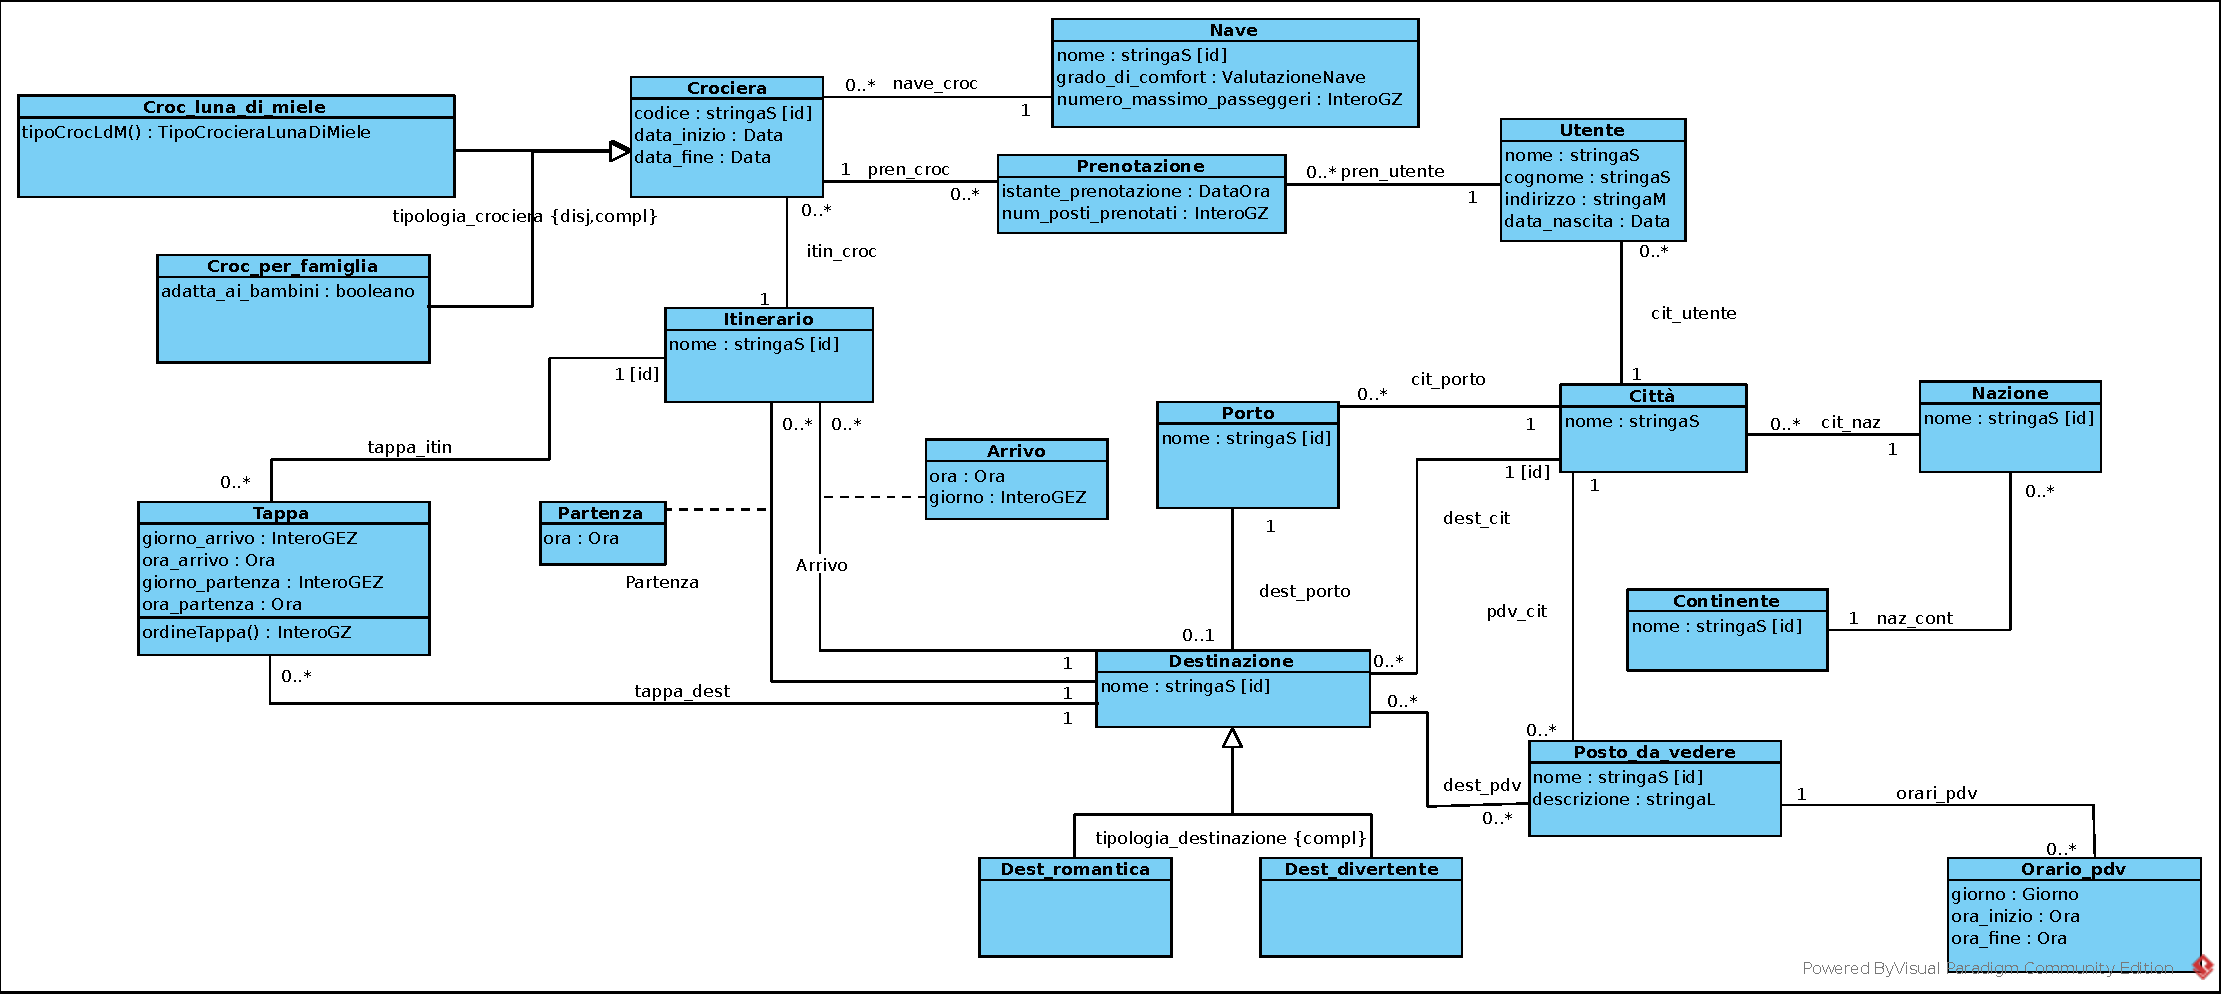
\includegraphics[width=\textwidth]{../Diagramma delle classi.pdf}
    \caption{Diagramma delle classi}
\end{figure}

\newpage
\section{Specifiche dei tipi di dati}

\begin{enumerate}
    \item ValutazioneNave Intero in [3,5]\label{sec:ValutazioneNave}
    \item InteroGEZ Intero in [0, +$\infty$]\label{sec:InteroGEZ}
    \item InteroGZ Intero in (0, +$\infty$)\label{sec:InteroGZ}
    \item Giorno \{Lun, Mar, Mer, Gio, Ven, Sab, Dom\}\label{sec:Giorno}
    \item DeltaOra \{ora: intero in [0,23], minuti: intero in [0,59]\}\label{sec:DeltaOra}
    \item StringaS varchar di lunghezza 100\label{sec:StringaS}
    \item StringaM varchar di lunghezza 500\label{sec:StringaM}
    \item StringaL varchar di lunghezza 1000\label{sec:StringaL}
    \item TipoCrocieraLunaDiMiele \{tradizionale, alternativa\}\label{sec:TipoCrocieraLunaDiMiele}
\end{enumerate}

Operazioni del tipo \hyperref[sec:DeltaOra]{DeltaOra}:\label{sec:OperazioniDeltaOra}

\begin{enumerate}
    \item $<$ (d1: \hyperref[sec:DeltaOra]{DeltaOra}, d2: \hyperref[sec:DeltaOra]{DeltaOra}): booleano
    \begin{enumerate}
        \item Pre: nessuna
        \item Post: no side effect
        \item Return:
        \begin{enumerate}
            \item se d1.ora $<$ d2.ora, restituisce vero
            \item se d1.ora = d2.ora e d1.minuti $<$ d2.minuti, restituisce vero
            \item altrimenti, restituisce falso
        \end{enumerate}
    \end{enumerate}
\end{enumerate}

\newpage
\section{Specifiche delle classi e delle associazioni}
\subsection*{Classe Crociera, \hyperref[sec:RequisitiCrociera]{v.req.1}}\label{sec:Crociera}
Tabella delle specifiche degli attributi:
\begin{table}[h!]
    \centering
    \begin{tabular}{|c|c|c|c|}
        \hline
        Attributo & Tipo & Cardinalità & Descrizione \\
        \hline
        codice & \hyperref[sec:StringaS]{StringaS} & 1 & Codice della crociera \\
        data\_inizio & Data & 1 & Data di inizio della crociera \\
        data\_fine & Data & 1 & Data di fine della crociera \\
        \hline
    \end{tabular}
    \caption{Attributi della classe Crociera}
\end{table}

Tabella delle specifiche delle associazioni:
\begin{table}[h!]
    \centering
    \begin{tabular}{|c|c|c|c|}
        \hline
        Associazione & Cardinalità & Descrizione \\
        \hline
        nave\_croc & 1 & La nave utilizzata per la crociera \\
        itin\_croc & 1 & L'itinerario della crociera \\
        pren\_croc & 0..* & Le prenotazioni della crociera \\
        \hline
    \end{tabular}
    \caption{Associazioni della classe Crociera}
\end{table}

\subsection*{Classe Croc\_luna\_di\_miele, \hyperref[sec:RequisitiCrocieraTipoLunaDiMiele]{v.req.1.7.1.}}\label{sec:Croc_luna_di_miele}
Tabella delle specifiche degli attributi:
\begin{table}[h!]
    \centering
    \begin{tabular}{|c|c|c|c|}
        \hline
        Attributo & Tipo & Cardinalità & Descrizione \\
        \hline
        tipo & \hyperref[sec:TipoCrocieraLunaDiMiele]{TipoCrocieraLunaDiMiele} & 1 & Tipo della crociera di luna di miele \\
        \hline
    \end{tabular}
    \caption{Attributi della classe Classe Croc\_luna\_di\_miele}
\end{table}

Specifica delle operazioni della classe Croc\_luna\_di\_miele:

tipCrocLdM$()$: \hyperref[sec:TipoCrocieraLunaDiMiele]{TipoCrocieraLunaDiMiele}
\begin{enumerate}
    \item Pre: nessuna
    \item Post: no side effect
    \item Return:
    \begin{enumerate}
        \item se il numero di destinazioni romantiche $\geq$ il numero di destinazioni divertenti, restituisce tradizionale
        \item altrimenti, restituisce alternativa
    \end{enumerate}
\end{enumerate}

Tabella delle specifiche delle associazioni:
\begin{table}[h!]
    \centering
    \begin{tabular}{|c|c|c|c|}
        \hline
        Associazione & Cardinalità & Descrizione \\
        \hline
        \hline
    \end{tabular}
    \caption{Associazioni della classe Classe Croc\_luna\_di\_miele}
\end{table}

\subsection*{Classe\ Croc\_per\_famiglie, \hyperref[sec:RequisitiCrocieraTipoPerFamiglie]{v.req.1.7.2.}}\label{sec:Croc_per_famiglie}

Tabella delle specifiche degli attributi:
\begin{table}[h!]
    \centering
    \begin{tabular}{|c|c|c|c|}
        \hline
        Attributo & Tipo & Cardinalità & Descrizione \\
        \hline
        adatta\_ai\_bambini & booleano & 1 & Indica se la crociera è adatta ai bambini \\
        \hline
    \end{tabular}
    \caption{Attributi della classe Classe Croc\_per\_famiglie}
\end{table}

Tabella delle specifiche delle associazioni:
\begin{table}[h!]
    \centering
    \begin{tabular}{|c|c|c|c|}
        \hline
        Associazione & Cardinalità & Descrizione \\
        \hline
    \end{tabular}
    \caption{Associazioni della classe Classe\ Croc\_per\_famiglie}
\end{table}

\subsection*{Classe Nave, \hyperref[sec:RequisitiNave]{v.req.2}}\label{sec:Nave}
Tabella delle specifiche degli attributi:
\begin{table}[h!]
    \centering
    \begin{tabular}{|c|c|c|c|}
        \hline
        Attributo & Tipo & Cardinalità & Descrizione \\
        \hline
        nome & \hyperref[sec:StringaS]{StringaS} & 1 & Nome della nave \\
        grado\_di\_comfort & \hyperref[sec:ValutazioneNave]{ValutazioneNave} & 1 & Grado di comfort della nave \\
        numero\_massimo\_di\_passeggeri & \hyperref[sec:InteroGZ]{InteroGZ} & 1 & Numero massimo di passeggeri \\
        \hline
    \end{tabular}
    \caption{Attributi della classe Nave}
\end{table}

Tabella delle specifiche delle associazioni:
\begin{table}[h!]
    \centering
    \begin{tabular}{|c|c|c|c|}
        \hline
        Associazione & Cardinalità & Descrizione \\
        \hline
        nave\_croc & 0..* & Le crociere che fanno uso della nave \\
        \hline
    \end{tabular}
    \caption{Associazioni della classe Nave}
\end{table}

\subsection*{Classe Destinazione, \hyperref[sec:RequisitiDestinazione]{v.req.3}}\label{sec:Destinazione}

Tabella delle specifiche degli attributi:
\begin{table}[h!]
    \centering
    \begin{tabular}{|c|c|c|c|}
        \hline
        Attributo & Tipo & Cardinalità & Descrizione \\
        \hline
        nome & \hyperref[sec:StringaS]{StringaS} & 1 & Nome della destinazione \\
        \hline
    \end{tabular}
    \caption{Attributi della classe Destinazione}
\end{table}

Tabella delle specifiche delle associazioni:
\begin{table}[h!]
    \centering
    \begin{tabular}{|c|c|c|c|}
        \hline
        Associazione & Cardinalità & Descrizione \\
        \hline
        dest\_cit & 1 & La città in cui si trova la destinazione \\
        dest\_pdv & 0..* & I posti da vedere della destinazione \\
        dest\_porto & 1 & Il porto dal quale può essere raggiunta la destinazione \\
        \hline
    \end{tabular}
    \caption{Associazioni della classe Destinazione}
\end{table}
\subsection*{Classe Itinerario, \hyperref[sec:RequisitiItinerario]{v.req.4}}\label{sec:Itinerario}

Tabella delle specifiche degli attributi:
\begin{table}[h!]
    \centering
    \begin{tabular}{|c|c|c|c|}
        \hline
        Attributo & Tipo & Cardinalità & Descrizione \\
        \hline
        nome & \hyperref[sec:StringaS]{StringaS} & 1 & Nome dell'itinerario \\
        \hline
    \end{tabular}
    \caption{Attributi della classe Itinerario}
\end{table}

Tabella delle specifiche delle associazioni:
\begin{table}[h!]
    \centering
    \begin{tabular}{|c|c|c|c|}
        \hline
        Associazione & Cardinalità & Descrizione \\
        \hline
        tappa\_itin & 1..* & Le tappe dell'itinerario \\
        itin\_croc & 0..* & Le crociere che prevedono l'itinerario \\
        partenza & 1 & La destinazione di partenza dell'itinerario \\
        arrivo & 1 & La destinazione di arrivo dell'itinerario \\
        \hline
    \end{tabular}
    \caption{Associazioni della classe Itinerario} 
\end{table}

\subsection*{Association Class Partenza, \hyperref[sec:RequisitiItinerarioDestinazioneDiPartenza]{v.req.4.3.}}

\begin{table}[h!]
    \centering
    \begin{tabular}{|c|c|c|c|}
        \hline
        Attributo & Tipo & Cardinalità & Descrizione \\
        \hline
        ora & \hyperref[sec:DeltaOra]{DeltaOra} & 1 & Ora di partenza \\
        \hline
    \end{tabular}
    \caption{Attributi dell'association class Partenza'}
\end{table}

\subsection*{Association Class Arrivo, \hyperref[sec:RequisitiItinerarioDestinazioneDiArrivo]{v.req.4.4.}}

\begin{table}[h!]
    \centering
    \begin{tabular}{|c|c|c|c|}
        \hline
        Attributo & Tipo & Cardinalità & Descrizione \\
        \hline
        ora & \hyperref[sec:DeltaOra]{DeltaOra} & 1 & Ora di arrivo \\
        giorno & \hyperref[sec:InteroGEZ]{InteroGEZ} & 1 & Giorno di arrivo \\
        \hline
    \end{tabular}
    \caption{Attributi dell'association class Arrivo'}
\end{table}

\subsection*{Classe PostoDaVedere, \hyperref[sec:RequisitiPostoDaVedere]{v.req.5}}\label{sec:PostoDaVedere}

Tabella delle specifiche degli attributi:
\begin{table}[h!]
    \centering
    \begin{tabular}{|c|c|c|c|}
        \hline
        Attributo & Tipo & Cardinalità & Descrizione \\
        \hline
        nome & \hyperref[sec:StringaS]{StringaS} & 1 & Nome del posto da vedere \\
        descrizione & \hyperref[sec:StringaL]{StringaL} & 1 & Descrizione del posto da vedere \\
        \hline
    \end{tabular}
    \caption{Attributi della classe Posto Da Vedere}
\end{table}

Tabella delle specifiche delle associazioni:
\begin{table}[h!]
    \centering
    \begin{tabular}{|c|c|c|c|}
        \hline
        Associazione & Cardinalità & Descrizione \\
        \hline
        pdv\_cit & 1 & La città in cui si trova il posto da vedere \\
        dest\_pdv & 0..* & Le destinazioni in cui si trova il posto da vedere \\
        orari\_pdv & 0..* & Gli orari del posto da vedere \\
        \hline
    \end{tabular}
    \caption{Associazioni della classe Posto Da Vedere}
\end{table}

\subsection*{Classe Utente, \hyperref[sec:RequisitiUtente]{v.req.6}}\label{sec:Utente}

Tabella delle specifiche degli attributi:
\begin{table}[h!]
    \centering
    \begin{tabular}{|c|c|c|c|}
        \hline
        Attributo & Tipo & Cardinalità & Descrizione \\
        \hline
        nome & \hyperref[sec:StringaS]{StringaS} & 1 & Nome dell'utente \\
        cognome & \hyperref[sec:StringaS]{StringaS} & 1 & Cognome dell'utente \\
        indirizzo & \hyperref[sec:StringaM]{StringaM} & 1 & Indirizzo dell'utente \\
        data\_di\_nascita & Data & 1 & Data di nascita dell'utente \\
        \hline
    \end{tabular}
    \caption{Attributi della classe Utente}
\end{table}

Tabella delle specifiche delle associazioni:
\begin{table}[h!]
    \centering
    \begin{tabular}{|c|c|c|c|}
        \hline
        Associazione & Cardinalità & Descrizione \\
        \hline
        pren\_utente & 0..* & Le prenotazioni effettuate dall'utente \\
        cit\_utente & 1 & La città di residenza dell'utente \\
        \hline
    \end{tabular}
    \caption{Associazioni della classe Utente}
\end{table}
\subsection*{Classe Prenotazione, \hyperref[sec:RequisitiPrenotazione]{v.req.7}}\label{sec:Prenotazione}

Tabella delle specifiche degli attributi:
\begin{table}[h!]
    \centering
    \begin{tabular}{|c|c|c|c|}
        \hline
        Attributo & Tipo & Cardinalità & Descrizione \\
        \hline
        istante\_prenotazione & Dataora & 1 & Istante di prenotazione \\
        num\_posti\_prenotati & \hyperref[sec:InteroGZ]{InteroGZ} & 1 & Numero di posti prenotati \\
        \hline
    \end{tabular}
    \caption{Attributi della classe Prenotazione}
\end{table}

Tabella delle specifiche delle associazioni:
\begin{table}[h!]
    \centering
    \begin{tabular}{|c|c|c|c|}
        \hline
        Associazione & Cardinalità & Descrizione \\
        \hline
        pren\_croc & 1 & La crociera prenotata \\
        pren\_utente & 1 & L'utente che ha effettuato la prenotazione \\
        \hline
    \end{tabular}
    \caption{Associazioni della classe Prenotazione}
\end{table}

\subsection*{Classe Città, \hyperref[sec:RequisitiCittà]{v.req.8}}\label{sec:Città}

Tabella delle specifiche degli attributi:
\begin{table}[h!]
    \centering
    \begin{tabular}{|c|c|c|c|}
        \hline
        Attributo & Tipo & Cardinalità & Descrizione \\
        \hline
        nome & \hyperref[sec:StringaS]{StringaS} & 1 & Nome della città \\
        \hline
    \end{tabular}
    \caption{Attributi della classe Città}
\end{table}

Tabella delle specifiche delle associazioni:
\begin{table}[h!]
    \centering
    \begin{tabular}{|c|c|c|c|}
        \hline
        Associazione & Cardinalità & Descrizione \\
        \hline
        cit\_naz & 1 & La nazione in cui si trova la città \\
        dest\_cit & 0..* & Le destinazioni che si trovano nella città \\
        pdv\_cit & 0..* & I posti da vedere che si trovano nella città \\
        cit\_porto & 0..* & I porti che si trovano nella città \\
        cit\_utente & 0..* & Gli utenti che risiedono nella città \\
        \hline
    \end{tabular}
    \caption{Associazioni della classe Città}
\end{table}
\subsection*{Classe Nazione, \hyperref[sec:RequisitiNazione]{v.req.9}}\label{sec:Nazione}

Tabella delle specifiche degli attributi:
\begin{table}[h!]
    \centering
    \begin{tabular}{|c|c|c|c|}
        \hline
        Attributo & Tipo & Cardinalità & Descrizione \\
        \hline
        nome & \hyperref[sec:StringaS]{StringaS} & 1 & Nome della nazione \\
        \hline
    \end{tabular}
    \caption{Attributi della classe Nazione}
\end{table}

Tabella delle specifiche delle associazioni:
\begin{table}[h!]
    \centering
    \begin{tabular}{|c|c|c|c|}
        \hline
        Associazione & Cardinalità & Descrizione \\
        \hline
        naz\_cont & 1 & Il continente in cui si trova la nazione \\
        cit\_naz & 0..* & Le città che si trovano nella nazione \\
        \hline
    \end{tabular}
    \caption{Associazioni della classe Nazione}
\end{table}
\subsection*{Classe Continente, \hyperref[sec:RequisitiContinente]{v.req.10}}\label{sec:Continente}

Tabella delle specifiche degli attributi:
\begin{table}[h!]
    \centering
    \begin{tabular}{|c|c|c|c|}
        \hline
        Attributo & Tipo & Cardinalità & Descrizione \\
        \hline
        nome & \hyperref[sec:StringaS]{StringaS} & 1 & Nome del continente \\
        \hline
    \end{tabular}
    \caption{Attributi della classe Continente}
\end{table}

Tabella delle specifiche delle associazioni:
\begin{table}[h!]
    \centering
    \begin{tabular}{|c|c|c|c|}
        \hline
        Associazione & Cardinalità & Descrizione \\
        \hline
        naz\_cont & 0..* & Le nazioni che si trovano nel continente \\
        \hline
    \end{tabular}
    \caption{Associazioni della classe Continente}
\end{table}

\subsection*{Classe Porto, \hyperref[sec:RequisitiPorto]{v.req.11}}\label{sec:Porto}

Tabella delle specifiche degli attributi:
\begin{table}[h!]
    \centering
    \begin{tabular}{|c|c|c|c|}
        \hline
        Attributo & Tipo & Cardinalità & Descrizione \\
        \hline
        nome & \hyperref[sec:StringaS]{StringaS} & 1 & Nome del porto \\
        \hline
    \end{tabular}
    \caption{Attributi della classe Porto}
\end{table}

Tabella delle specifiche delle associazioni:
\begin{table}[h!]
    \centering
    \begin{tabular}{|c|c|c|c|}
        \hline
        Associazione & Cardinalità & Descrizione \\
        \hline
        cit\_porto & 1 & La città in cui si trova il porto \\
        dest\_porto & 0..1 & La destinazione che può essere raggiunta dal porto \\
        \hline
    \end{tabular}
    \caption{Associazioni della classe Porto}
\end{table}
\subsection*{Classe OrarioPostoDaVedere, \hyperref[sec:RequisitiOrarioPostoDaVedere]{v.req.12}}\label{sec:OrarioPostoDaVedere}
Tabella delle specifiche degli attributi:
\begin{table}[h!]
    \centering
    \begin{tabular}{|c|c|c|c|}
        \hline
        Attributo & Tipo & Cardinalità & Descrizione \\
        \hline
        giorno & \hyperref[sec:Giorno]{Giorno} & 1 & Giorno in cui è possibile visitare il posto \\
        ora\_inizio & \hyperref[sec:DeltaOra]{DeltaOra} & 1 & Ora di inizio della visita \\
        ora\_fine & \hyperref[sec:DeltaOra]{DeltaOra} & 1 & Ora di fine della visita \\
        \hline
    \end{tabular}
    \caption{Attributi della classe Orario Posto Da Vedere}
\end{table}

Tabella delle specifiche delle associazioni:
\begin{table}[h!]
    \centering
    \begin{tabular}{|c|c|c|c|}
        \hline
        Associazione & Cardinalità & Descrizione \\
        \hline
        orari\_pdv & 1 & Il posto da vedere per il quale è definito l'orario \\
        \hline
    \end{tabular}
    \caption{Associazioni della classe Orario Posto Da Vedere}
\end{table}

\subsection*{Classe Tappa, \hyperref[sec:RequisitiTappa]{v.req.13}}\label{sec:Tappa}

Tabella delle specifiche degli attributi:
\begin{table}[h!]
    \centering
    \begin{tabular}{|c|c|c|c|}
        \hline
        Attributo & Tipo & Cardinalità & Descrizione \\
        \hline
        giorno\_arrivo & \hyperref[sec:InteroGEZ]{InteroGEZ} & 1 & Giorno di arrivo della tappa \\
        ora\_arrivo & \hyperref[sec:DeltaOra]{DeltaOra} & 1 & Ora di arrivo della tappa \\
        giorno\_partenza & \hyperref[sec:InteroGEZ]{InteroGEZ} & 1 & Giorno di partenza della tappa \\
        ora\_partenza & \hyperref[sec:DeltaOra]{DeltaOra} & 1 & Ora di partenza della tappa \\
        \hline
    \end{tabular}
    \caption{Attributi della classe Tappa}
\end{table}

Specifica delle operazioni della classe Tappa:

ordineTappa(): \hyperref[sec:InteroGZ]{InteroGZ}
\begin{enumerate}
    \item Pre: nessuna
    \item Post: no side effect
    \item Return:
    \begin{enumerate}
        \item sia I l'itinerario tale che tappa\_itin(this, I) = True
        \item sia T l'insieme delle tappe di I
        \item sia T' = \{t' $\in$ T: (giorno\_arrivo(t') $\leq$ giorno\_arrivo(t)) \newline $\lor$ (giorno\_arrivo(t') = giorno\_arrivo(t) $\land$ ora\_partenza(t') $\leq$ ora\_arrivo(t))\}
        \item restituisce la cardinalità di T'+1
    \end{enumerate}
\end{enumerate}


Tabella delle specifiche delle associazioni:
\begin{table}[h!]
    \centering
    \begin{tabular}{|c|c|c|c|}
        \hline
        Associazione & Cardinalità & Descrizione \\
        \hline
        tappa\_itin & 1 & L'itinerario della tappa \\
        tappa\_dest & 1 & La destinazione della tappa \\
        \hline
    \end{tabular}
    \caption{Associazioni della classe Tappa}
\end{table}

\newpage
\section{Specifiche dei vincoli esterni}

\section*{[V.\hyperref[sec:Crociera]{Crociera}.]}
    [V.Crociera.data\_inizio\_leq\_data\_fine.]:
    \begin{enumerate}
        \item data di inizio $\leq$ data di fine
    \end{enumerate}
    [V.Crociera.prenotazioni\_leq\_numero\_massimo\_passeggeri.]
    \begin{enumerate}
        \item La somma dei posti prenotati per la crociera $\leq$ numero massimo di passeggeri
    \end{enumerate}
\section*{[V.\hyperref[sec:Nave]{Nave}.]}
\section*{[V.\hyperref[sec:Destinazione]{Destinazione}.]}
\section*{[V.\hyperref[sec:Itinerario]{Itinerario}.]}
\section*{[V.\hyperref[sec:PostoDaVedere]{PostoDaVedere}.]}
\section*{[V.\hyperref[sec:Utente]{Utente}.]}
\section*{[V.\hyperref[sec:Prenotazione]{Prenotazione}.]}
    [V.Prenotazione.istante\_di\_prenotazione\_less\_data\_inizio\_crociera.]
    \begin{enumerate}
        \item istante di prenotazione $<$ data di inizio crociera
    \end{enumerate}
\section*{[V.\hyperref[sec:Città]{Città}.]}
\section*{[V.\hyperref[sec:Nazione]{Nazione}.]}
\section*{[V.\hyperref[sec:Continente]{Continente}.]}
\section*{[V.\hyperref[sec:Porto]{Porto}.]}
\section*{[V.\hyperref[sec:OrarioPostoDaVedere]{OrarioPostoDaVedere}.]}
    [V.OrarioPostoDaVedere.ora\_inizio\_less\_ora\_fine.]
    \begin{enumerate}
        \item ora di inizio $<$ ora di fine
    \end{enumerate}
\section*{[V.\hyperref[sec:Tappa]{Tappa}.]}
    [V.Tappa.giorno\_arrivo\_leq\_giorno\_partenza.]
    \begin{enumerate}
        \item giorno di arrivo $\leq$ giorno di partenza
    \end{enumerate}

\newpage
\section{Specifiche delle operazioni}

In questa sezione verranno descritte le operazioni che il sistema deve essere in grado di eseguire.
\newline
[getPostiDisponibili$($Crociera c$)$]
\begin{enumerate}
    \item Restituisce il numero di posti disponibili data una determinata Crociera.
\end{enumerate}
\space

[effettuaPrenotazione$($Crociera c, Utente u, InteroGZ num\_posti$)$]
\begin{enumerate}
    \item Permette all'Ufficio Prenotazioni di effettuare una prenotazione. Restituisce un oggetto di tipo Prenotazione se getPostiDisponibili$(c)$ $\geq$ num\_posti, altrimenti rifiuta.
\end{enumerate}

[isDestinazioneEsotica$($Destinazione d$)$]
\begin{enumerate}
    \item Restituisce vero se la destinazione è esotica (se il suo continente è diverso da Europa), altrimenti falso.
\end{enumerate}
\space

[isPrenotazioneInPeriodo$($Prenotazione p, Data inizio, Data fine$)$]
\begin{enumerate}
    \item Restituisce vero se la prenotazione è in un periodo compreso tra inizio e fine, altrimenti falso.
\end{enumerate}
\space

[getEtàMediaUtenti$($Utente[] u$)$]
\begin{enumerate}
    \item Restituisce l'età media degli utenti.
\end{enumerate}
\space

[getEtàMediaClientiCheHannoPrenotatoInUnPeriodoUnaCrocieraConAlmenoUnaDestinazioneEsotica$($Data inizio, Data fine$)$]
\begin{enumerate}
    \item Restituisce l'età media dei clienti che hanno prenotato in un periodo una crociera con almeno una destinazione esotica.
\end{enumerate}
\space

[getDestinazioniGettonateInUnDatoPeriodo$($Data inizio, Data fine$)$]
\begin{enumerate}
    \item Restituisce il numero di destinazioni da considerarsi gettonate in un dato periodo. Una destinazione è gettonata se è raggiunta da almeno 10 crociere luna di miele in quel periodo oppure da almeno 15 crociere per famiglia.
    \item D = l'insieme di tutte le destinazioni
    \item R = $\{d \in D: isDestinazioneGettonataInUnDatoPeriodo(d, inizio, fine)\}$
    \item return R
\end{enumerate}
\space

[isDestinazioneGettonataInUnDatoPeriodo$($Destinazione d, Data inizio, Data fine$)$]
\begin{enumerate}
    \item Restituisce vero se la destinazione è gettonata in un dato periodo, altrimenti falso.
    \item CpF = getCrocieraPerFamiglieCheRaggiungeUnaDataDestinazioneInUnDatoPeriodo$($d, inizio, fine$)$
    \item CLdM = getCrocieraLunaDiMieleCheRaggiungeUnaDataDestinazioneInUnDatoPeriodo$($d, inizio, fine$)$
    \item return True se cardinalità di CpF $\geq$ 15 $\lor$ cardinalità di CLdM $\geq$ 10, altrimenti False
\end{enumerate}
\space

[getCrocieraPerFamiglieCheRaggiungeUnaDataDestinazioneInUnDatoPeriodo$($Destinazione d, Data inizio, Data fine$)$]
\begin{enumerate}
    \item Restituisce le crociere per famiglie che raggiungono una data destinazione in un dato periodo.
    \item P = getCrocierePerFamiglieInUnDatoPeriodo$($inizio, fine$)$
    \item D = getCrocierePerFamiglieInDestinazione$($d$)$
    \item return P $\cap$ D
\end{enumerate}
\space

[getCrocieraLunaDiMieleCheRaggiungeUnaDataDestinazioneInUnDatoPeriodo$($Destinazione d, Data inizio, Data fine$)$]
\begin{enumerate}
    \item Restituisce le crociere luna di miele che raggiungono una data destinazione in un dato periodo.
    \item P = getCrociereLunaDiMieleInUnDatoPeriodo$($inizio, fine$)$
    \item D = getCrociereLunaDiMieleInDestinazione$($d$)$
    \item return P $\cap$ D
\end{enumerate}
\space

[isCrocieraInPeriodo$($Crociera c, Data inizio, Data fine$)$]
\begin{enumerate}
    \item Restituisce vero se la crociera è in un periodo compreso tra inizio e fine, altrimenti falso.
    \item return true se data\_inizio$($c$)$ $\geq$ inizio $\land$ data\_fine$($c$)$ $\leq$ fine, altrimenti false
\end{enumerate}
\space

[getPercentualeDestinazioniGettonateInUnDatoPeriodo$($Data inizio, Data fine$)$]
\begin{enumerate}
    \item Restituisce la percentuale di destinazioni gettonate in un dato periodo.
    \item D = l'insieme di tutte le destinazioni
    \item R = getDestinazioniGettonateInUnDatoPeriodo$($inizio, fine$)$
    \item return R*100/D
\end{enumerate}
\space

[getCrocierePerFamiglieInUnDatoPeriodo$($Data inizio, Data fine$)$]
\begin{enumerate}
    \item Restituisce le crociere per famiglie in un dato periodo.
    \item return $\{c \in Crociere: isCrocieraInPeriodo(c, inizio, fine) \land c \in CrocierePerFamiglie\}$
\end{enumerate}
\space

[getCrociereLunaDiMieleInUnDatoPeriodo$($Data inizio, Data fine$)$]
\begin{enumerate}
    \item Restituisce le crociere luna di miele in un dato periodo.
    \item return $\{c \in Crociere: isCrocieraInPeriodo(c, inizio, fine) \land c \in CrociereLunaDiMiele\}$
\end{enumerate}
\space

[getCrociereLunaDiMieleInDestinazione$($Destinazione d$)$]
\begin{enumerate}
    \item Restituisce le crociere luna di miele che raggiungono una data destinazione.
    \item return $\{c \in CrociereLunaDiMiele: isCrocieraInDestinazione(c, d)\}$
\end{enumerate}
\space

[getCrocierePerFamiglieInDestinazione$($Destinazione d$)$]
\begin{enumerate}
    \item Restituisce le crociere per famiglie che raggiungono una data destinazione.
    \item return $\{c \in CrocierePerFamiglie: isCrocieraInDestinazione(c, d)\}$
\end{enumerate}
\space

[isCrocieraInDestinazione$($Crociera c, Destinazione d$)$]
\begin{enumerate}
    \item Restituisce vero se la crociera raggiunge la destinazione, altrimenti falso.
    \item return true se esistono i, t tale che tappa\_itin$(t, i)$ $\land$ tappa\_dest$(t, d)$ $\land$ itin\_croc$(i, c)$
    \item $\lor$ se esiste i tale che arrivo$($i, d$)$ $\land$ itin\_croc$($i, c$)$
    \item $\lor$ se esiste i tale che partenza$($i, d$)$ $\land$ itin\_croc$($i, c$)$
    \item altrimenti false
\end{enumerate}

\end{document}